\documentclass[a4paper,11pt,openany]{book}
\usepackage[utf8]{inputenc}
\usepackage[left=2.54cm,top=2.54cm,right=2.54cm,bottom=2.54cm]{geometry}
\usepackage[spanish]{babel}
\usepackage{amsmath}
\usepackage{amsfonts}
\usepackage{amssymb}
\usepackage{graphicx}
\usepackage{color}
\usepackage[usenames,dvipsnames]{xcolor}
\usepackage{pifont}
\usepackage{marvosym}
\newtheorem{teo}{Teorema}
\newtheorem{ejemplo}{Ejemplo}
\newtheorem{defi}{Definición}
\newtheorem{coro}{Corolario}
\newtheorem{prueba}{Prueba}
\newtheorem{exmp}{Example}[section]
\newtheorem{ejer}{Ejercicio}[section]
\def\proof{\paragraph{\textsf{Demostración.} }}
\def\endproof{\hfill $\blacksquare$ \\}
\usepackage{multirow, array} % para las tablas
\usepackage{multirow}
\usepackage{tabularx}
\usepackage{float} % para usar [H]
\usepackage{tikz}
\usepackage[all]{xy}
\usepackage{cancel}
\usetikzlibrary{positioning}
\usepackage{enumitem}
\newcommand*{\itembolasazules}[1]{% bolas 3D
\footnotesize\protect\tikz[baseline=-3pt]%
\protect\node[scale=.7, circle, shade, ball
color=green]{\color{white}\Large\bf#1};}
\usepackage{tcolorbox} 
\tcbuselibrary{listingsutf8}
\newtcolorbox[auto counter,number within=section]{example}[2][]
{colback=green!5!white,colframe=green!75!black,fonttitle=\bfseries, title=Ejercicio~\thetcbcounter: #2,#1}
\usepackage{background}
\backgroundsetup{
placement=center,
angle=0,
scale=1.1,
contents= {{
\includegraphics{HojaCuadriculada.png}}}
}
 
 
\begin{document}
\begin{titlepage}
 
\begin{center}
\vspace*{-1in}
\begin{figure}[htb]
\begin{center}

\includegraphics[width=7cm]{ETITC.png}
\end{center}
\end{figure}
 
 
{\sc \huge Escuela Tecnológica Instituto Técnico Central (ETITC)}\\
\vspace*{0.15in}
Facultad de sistemas\\
\vspace*{0.6in}
\begin{Large}
\textbf{Taller 1: Operaciones Básicas con Números Complejos} \\
\textbf{Matem{\'a}ticas Especiales}\\
\end{Large}
\vspace*{0.3in}
\begin{large}
{\bf Autores} \\
 
\ 
 
Sergio Alejandro Enrrique Caballero Leon\\ 
Johan Alejandro Sogamoso Camacho \\ 
David Andrés Valero Vanegas \\ 
\end{large}
\vspace*{0.3in}
 
\end{center}
 
\begin{center}
{\bf Presentado a:} \\
 
\ 
 
Carlos Romero \\
 
\
 
Bogot{\'a}, 21 de Agosto de 2022.
\end{center}
 
\end{titlepage}

\newpage

\definecolor{ao(english)}{rgb}{0.0, 0.5, 0.0}

\begin{center}
\textbf{Gráfica y Módulo}
\end{center}

Dado los números $\bf{z_{1}}$ y $\bf{z_{2}}$, en cada uno de los ejercicios \ding{172} al \ding{174} grafique en un plano complejo los números $\bf{z_{1}}$, $\bf{z_{2}}$, $\bf{z_{1}\,+\,z_{2}}$ y $\bf{z_{1}\,-\,z_{2}}$. Finalmente calcule el módulo de los cuatro números.\\

\providecommand{\abs}[1]{\lvert#1\rvert} 
\graphicspath{ {images/} }




\textcolor{ao(english)}{\ding{172}}\,\quad\,$\bf{z_{1}\,=\,6\,-\,2\,i \quad\,;\,\quad z_{2}\,=\,2\,-\,5\,i}$

$$\,{z_1}\,+\,{z_2}\,=\,8\,-\,7\,i$$
$$\,{z_1}\,-\,{z_2}\,=\,4\,+\,3\,i$$

$$\abs{z_1} = \sqrt{\,(\,6\,)\,^{\,2}\,+\,(\,-\,2\,)\,^{\,2}\,}\,=\,\sqrt{\,36\,+\,4\,}\,=\,\boxed{2\sqrt{10}}$$

$$\abs{z_2} = \sqrt{\,(\,2\,)\,^{\,2}\,+\,(\,-\,5\,)\,^{\,2}\,}\,=\,\boxed{\sqrt{29}}$$

$$\abs{z_1\,+\,{z_2}\,} = \sqrt{\,(\,8\,)\,^{\,2}\,+\,(\,-\,7\,)\,^{\,2}\,}\,=\,\sqrt{\,64\,+\,49\,}\,=\,\boxed{\sqrt{113}}$$

$$\abs{z_1\,-\,{z_2}\,} = \sqrt{\,(\,4\,)\,^{\,2}\,+\,(\,-\,3\,)\,^{\,2}\,}\,=\,\sqrt{\,16\,+\,9\,}\,=\,\,\sqrt{\,25\,}\,=\,\boxed{5}$$

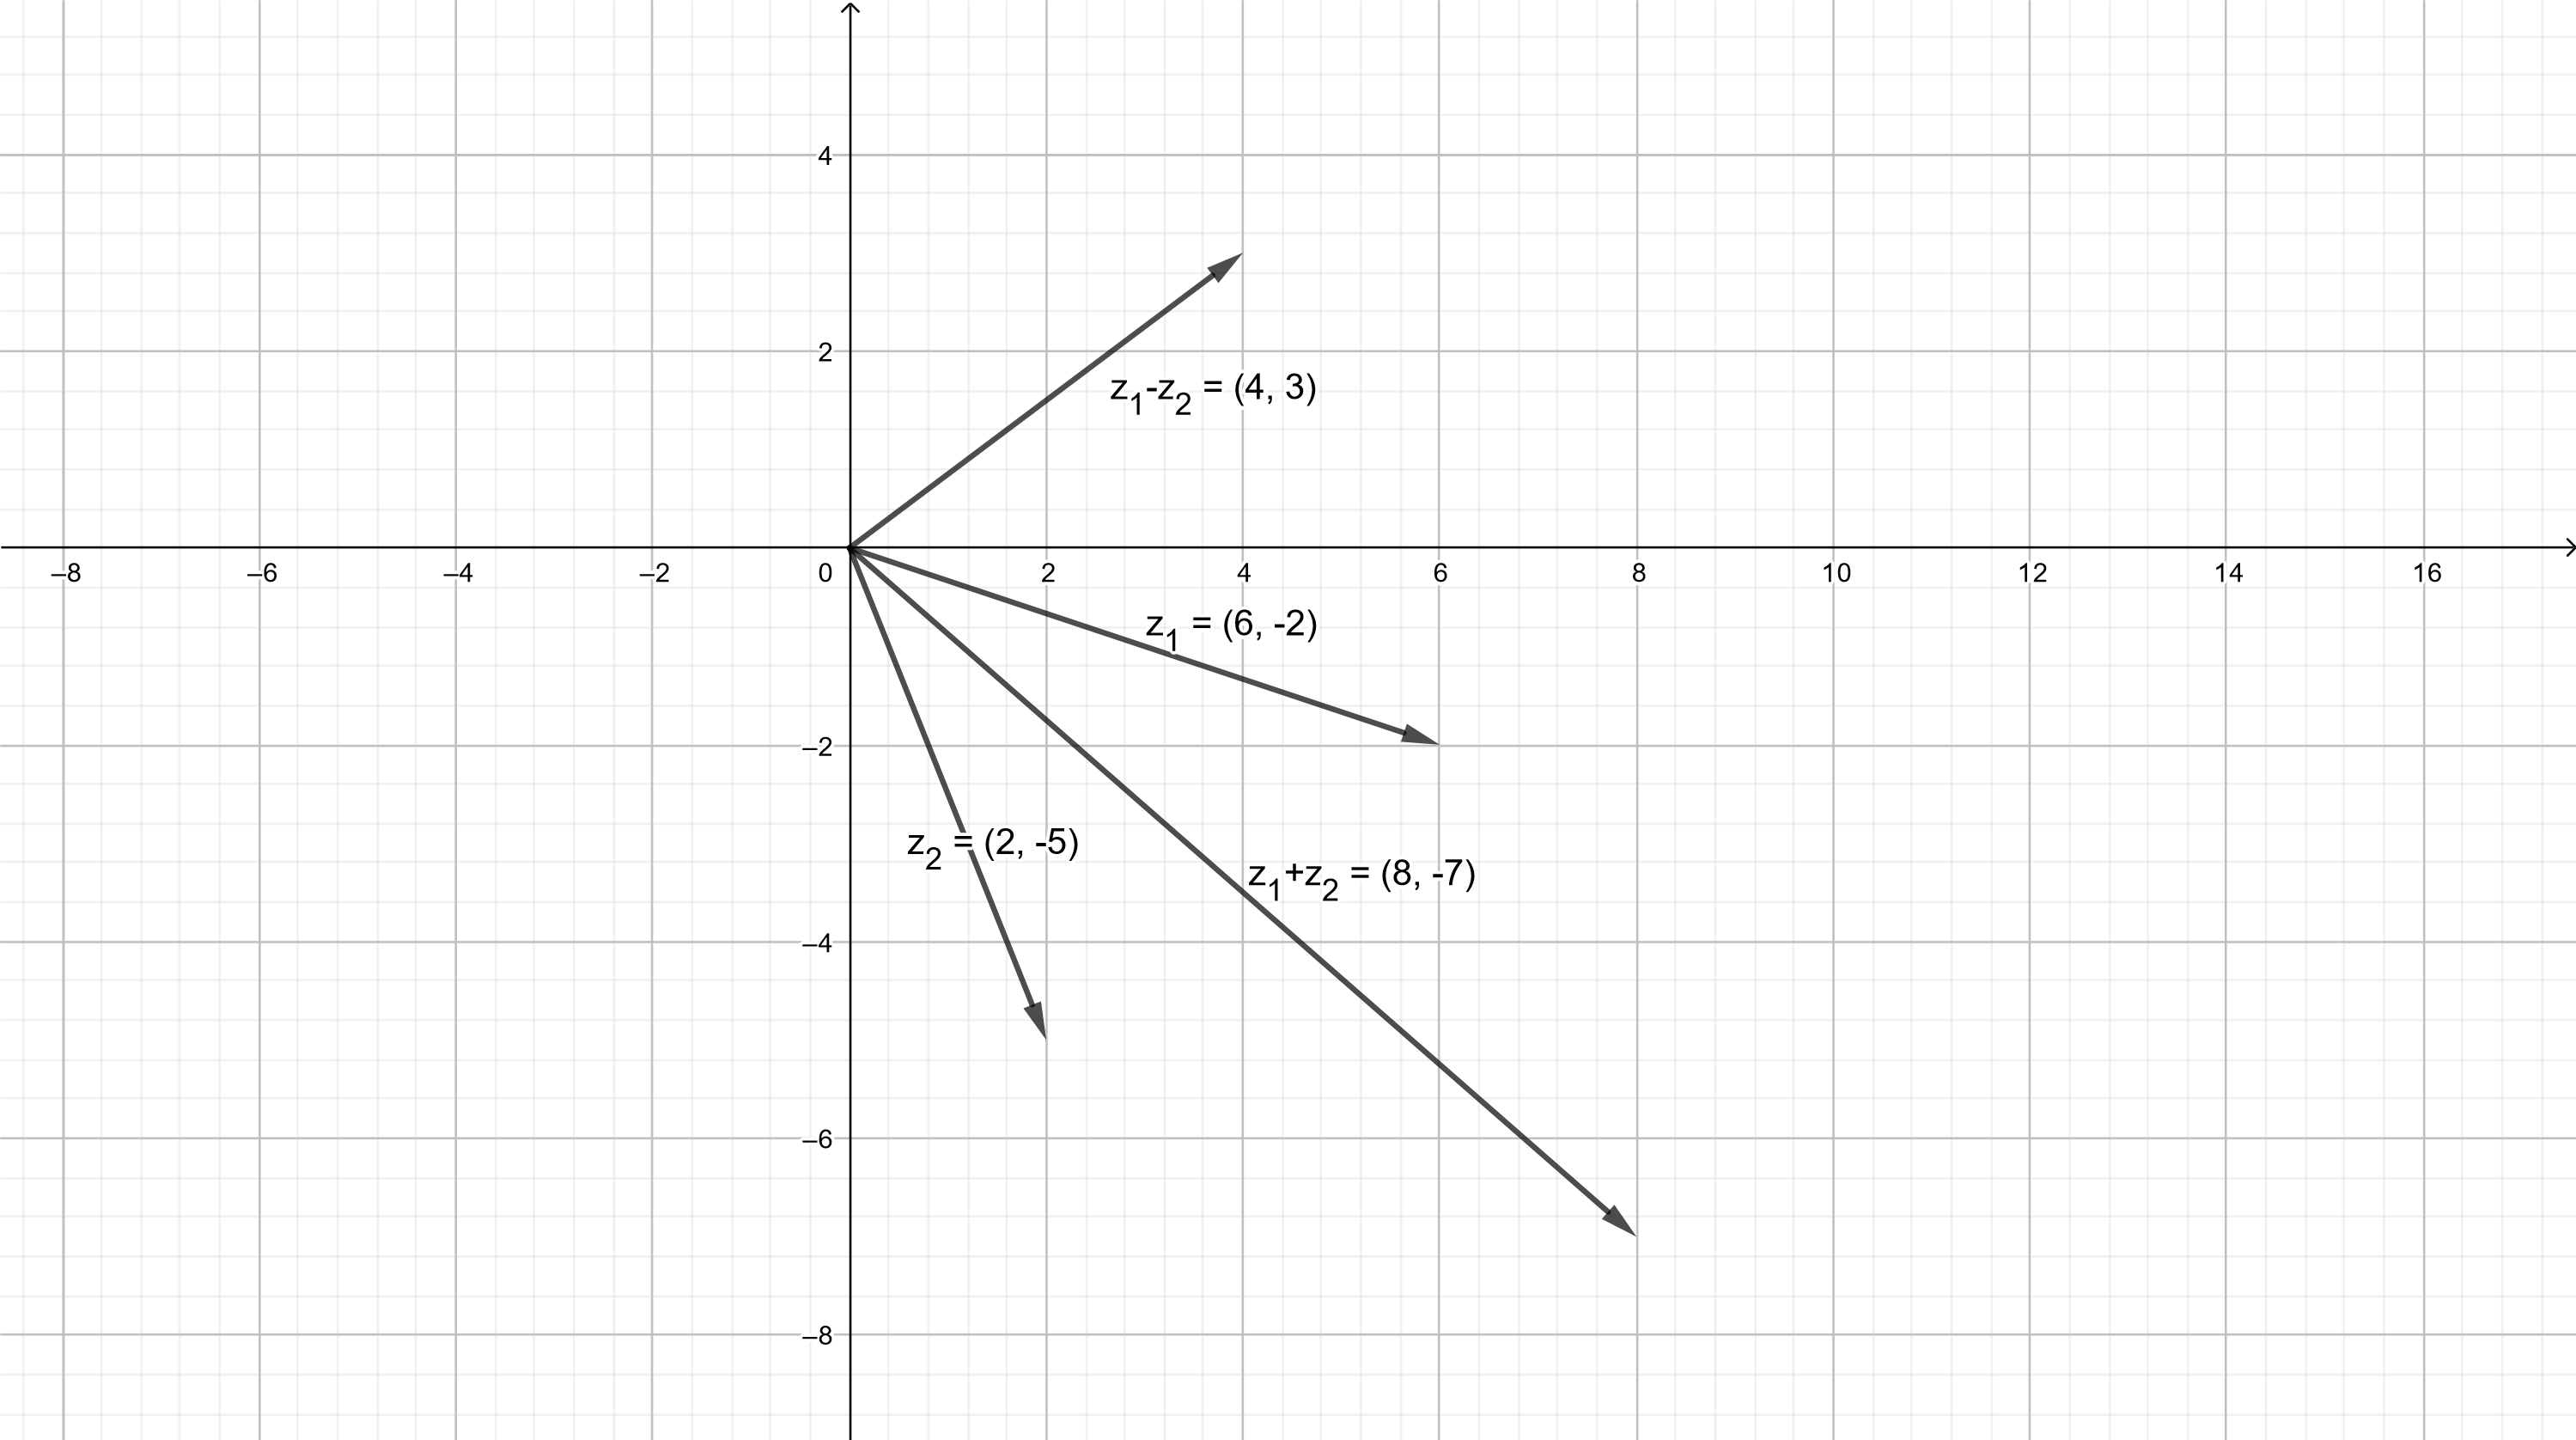
\includegraphics[width=15cm]{geo1}

\
\textcolor{ao(english)}{\ding{173}}\,\quad\,$\bf{z_{1}\,=\,-\,5\,+\,5\,i \quad\,;\,\quad z_{2}\,=\,-\,6\,-\,4\,i}$

$$\,{z_1}\,+\,{z_2}\,=\,-\,11\,+\,i$$
$$\,{z_1}\,-\,{z_2}\,=\,1\,+\,9\,i$$

$$\abs{z_1} = \sqrt{\,(\,5\,)\,^{\,2}\,+\,(\,-\,5\,)\,^{\,2}\,}\,=\,\sqrt{\,25\,+\,25\,}\,=\,\boxed{5\sqrt{2}}$$

$$\abs{z_2} = \sqrt{\,(\,-\,6\,)\,^{\,2}\,+\,(\,-\,4\,)\,^{\,2}\,}\,=\,\sqrt{\,36\,+\,16\,}\,=\,\boxed{2\sqrt{13}}$$

$$\abs{z_1\,+\,{z_2}\,} = \sqrt{\,(\,-\,11\,)\,^{\,2}\,+\,(\,1\,)\,^{\,2}\,}\,=\,\sqrt{\,121\,+\,1\,}\,=\,\boxed{\sqrt{122}}$$

$$\abs{z_1\,-\,{z_2}\,} = \sqrt{\,(\,1\,)\,^{\,2}\,+\,(\,9\,)\,^{\,2}\,}\,=\,\sqrt{\,1\,+\,81\,}\,=\,\,\boxed{\sqrt{82}}$$

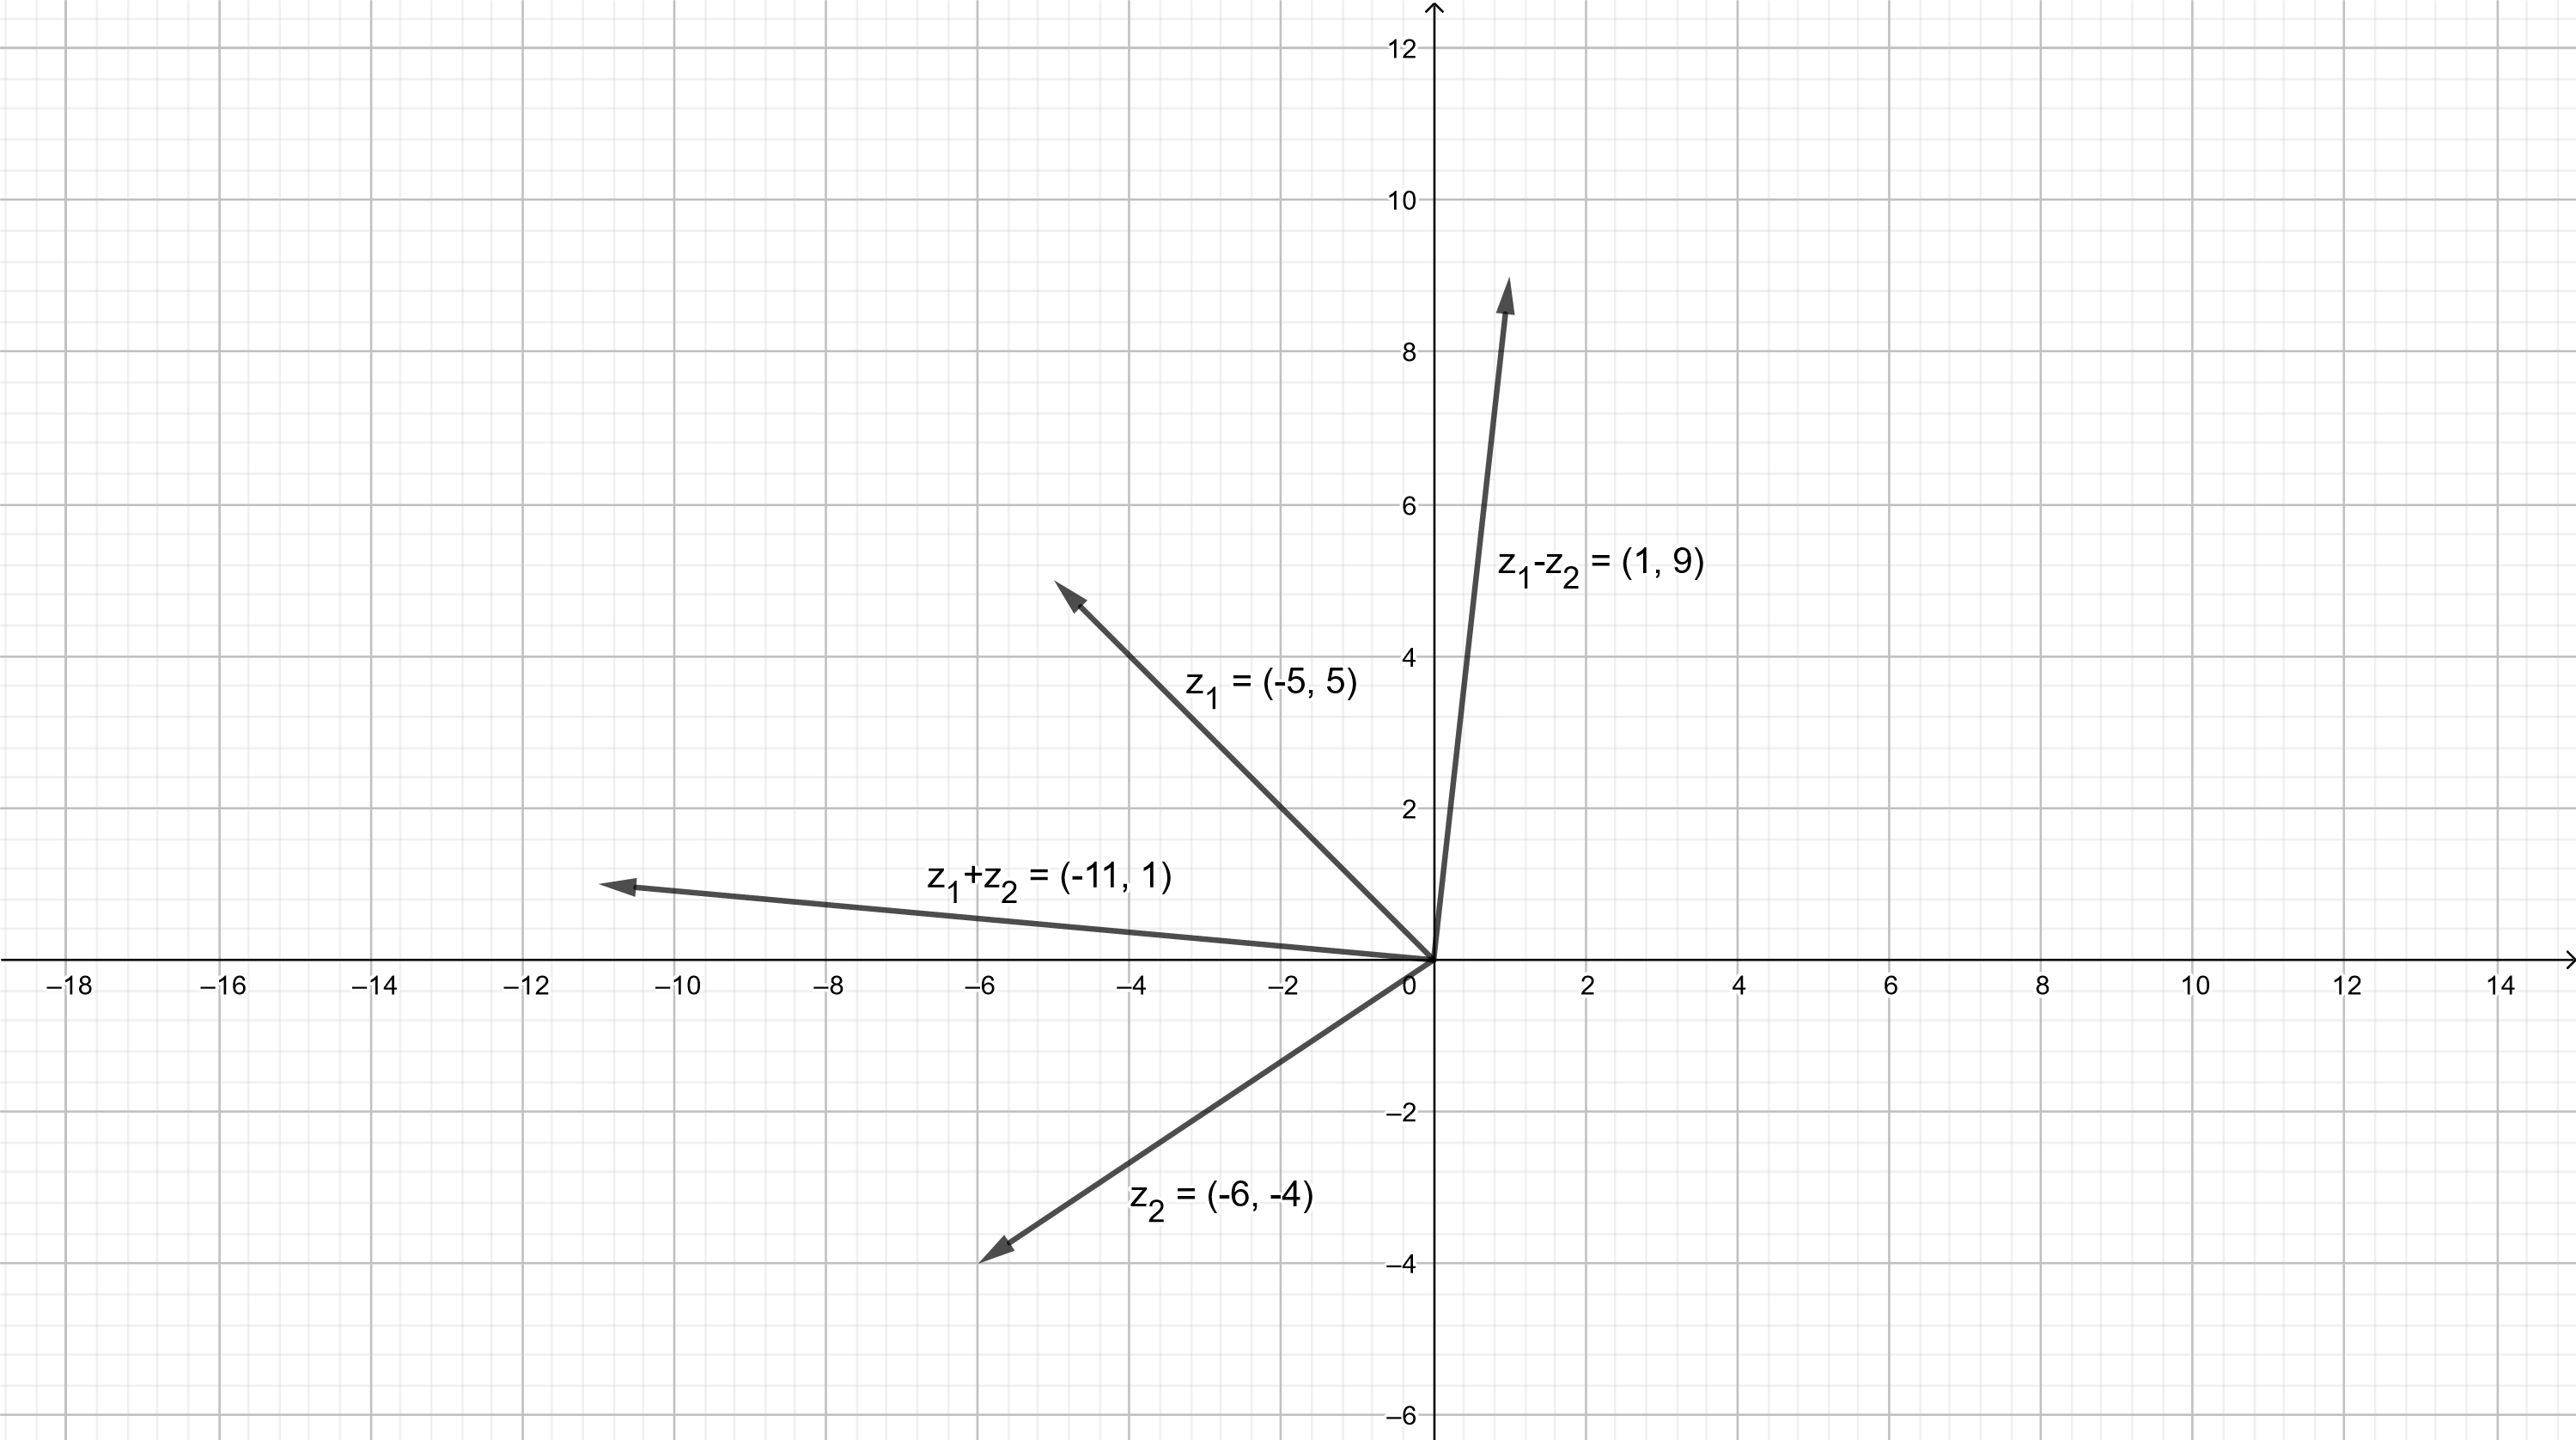
\includegraphics[width=15cm]{geo2}

\textcolor{ao(english)}{\ding{174}}\,\quad\,$\bf{z_{1}\,=\,8\,-\,6\,i \quad\,;\,\quad z_{2}\,=\,-\,4\,-\,8\,i}$

$$\,{z_1}\,+\,{z_2}\,=\,4\,-\,14\,i$$
$$\,{z_1}\,-\,{z_2}\,=\,12\,+\,2\,i$$

$$\abs{z_1} = \sqrt{\,(\,8\,)\,^{\,2}\,+\,(\,-\,6\,)\,^{\,2}\,}\,=\,\sqrt{\,64\,+\,36\,}\,=\,\boxed{10}$$

$$\abs{z_2} = \sqrt{\,(\,4\,)\,^{\,2}\,+\,(\,-\,8\,)\,^{\,2}\,}\,=\,\sqrt{\,16\,+\,64\,}\,=\,\boxed{4\sqrt{5}}$$

$$\abs{z_1\,+\,{z_2}\,} = \sqrt{\,(\,4\,)\,^{\,2}\,+\,(\,-\,14\,)\,^{\,2}\,}\,=\,\sqrt{\,16\,+\,196\,}\,=\,\boxed{2\sqrt{53}}$$

$$\abs{z_1\,-\,{z_2}\,} = \sqrt{\,(\,12\,)\,^{\,2}\,+\,(\,2\,)\,^{\,2}\,}\,=\,\sqrt{\,144\,+\,4\,}\,=\,\,\boxed{2\sqrt{37}}$$

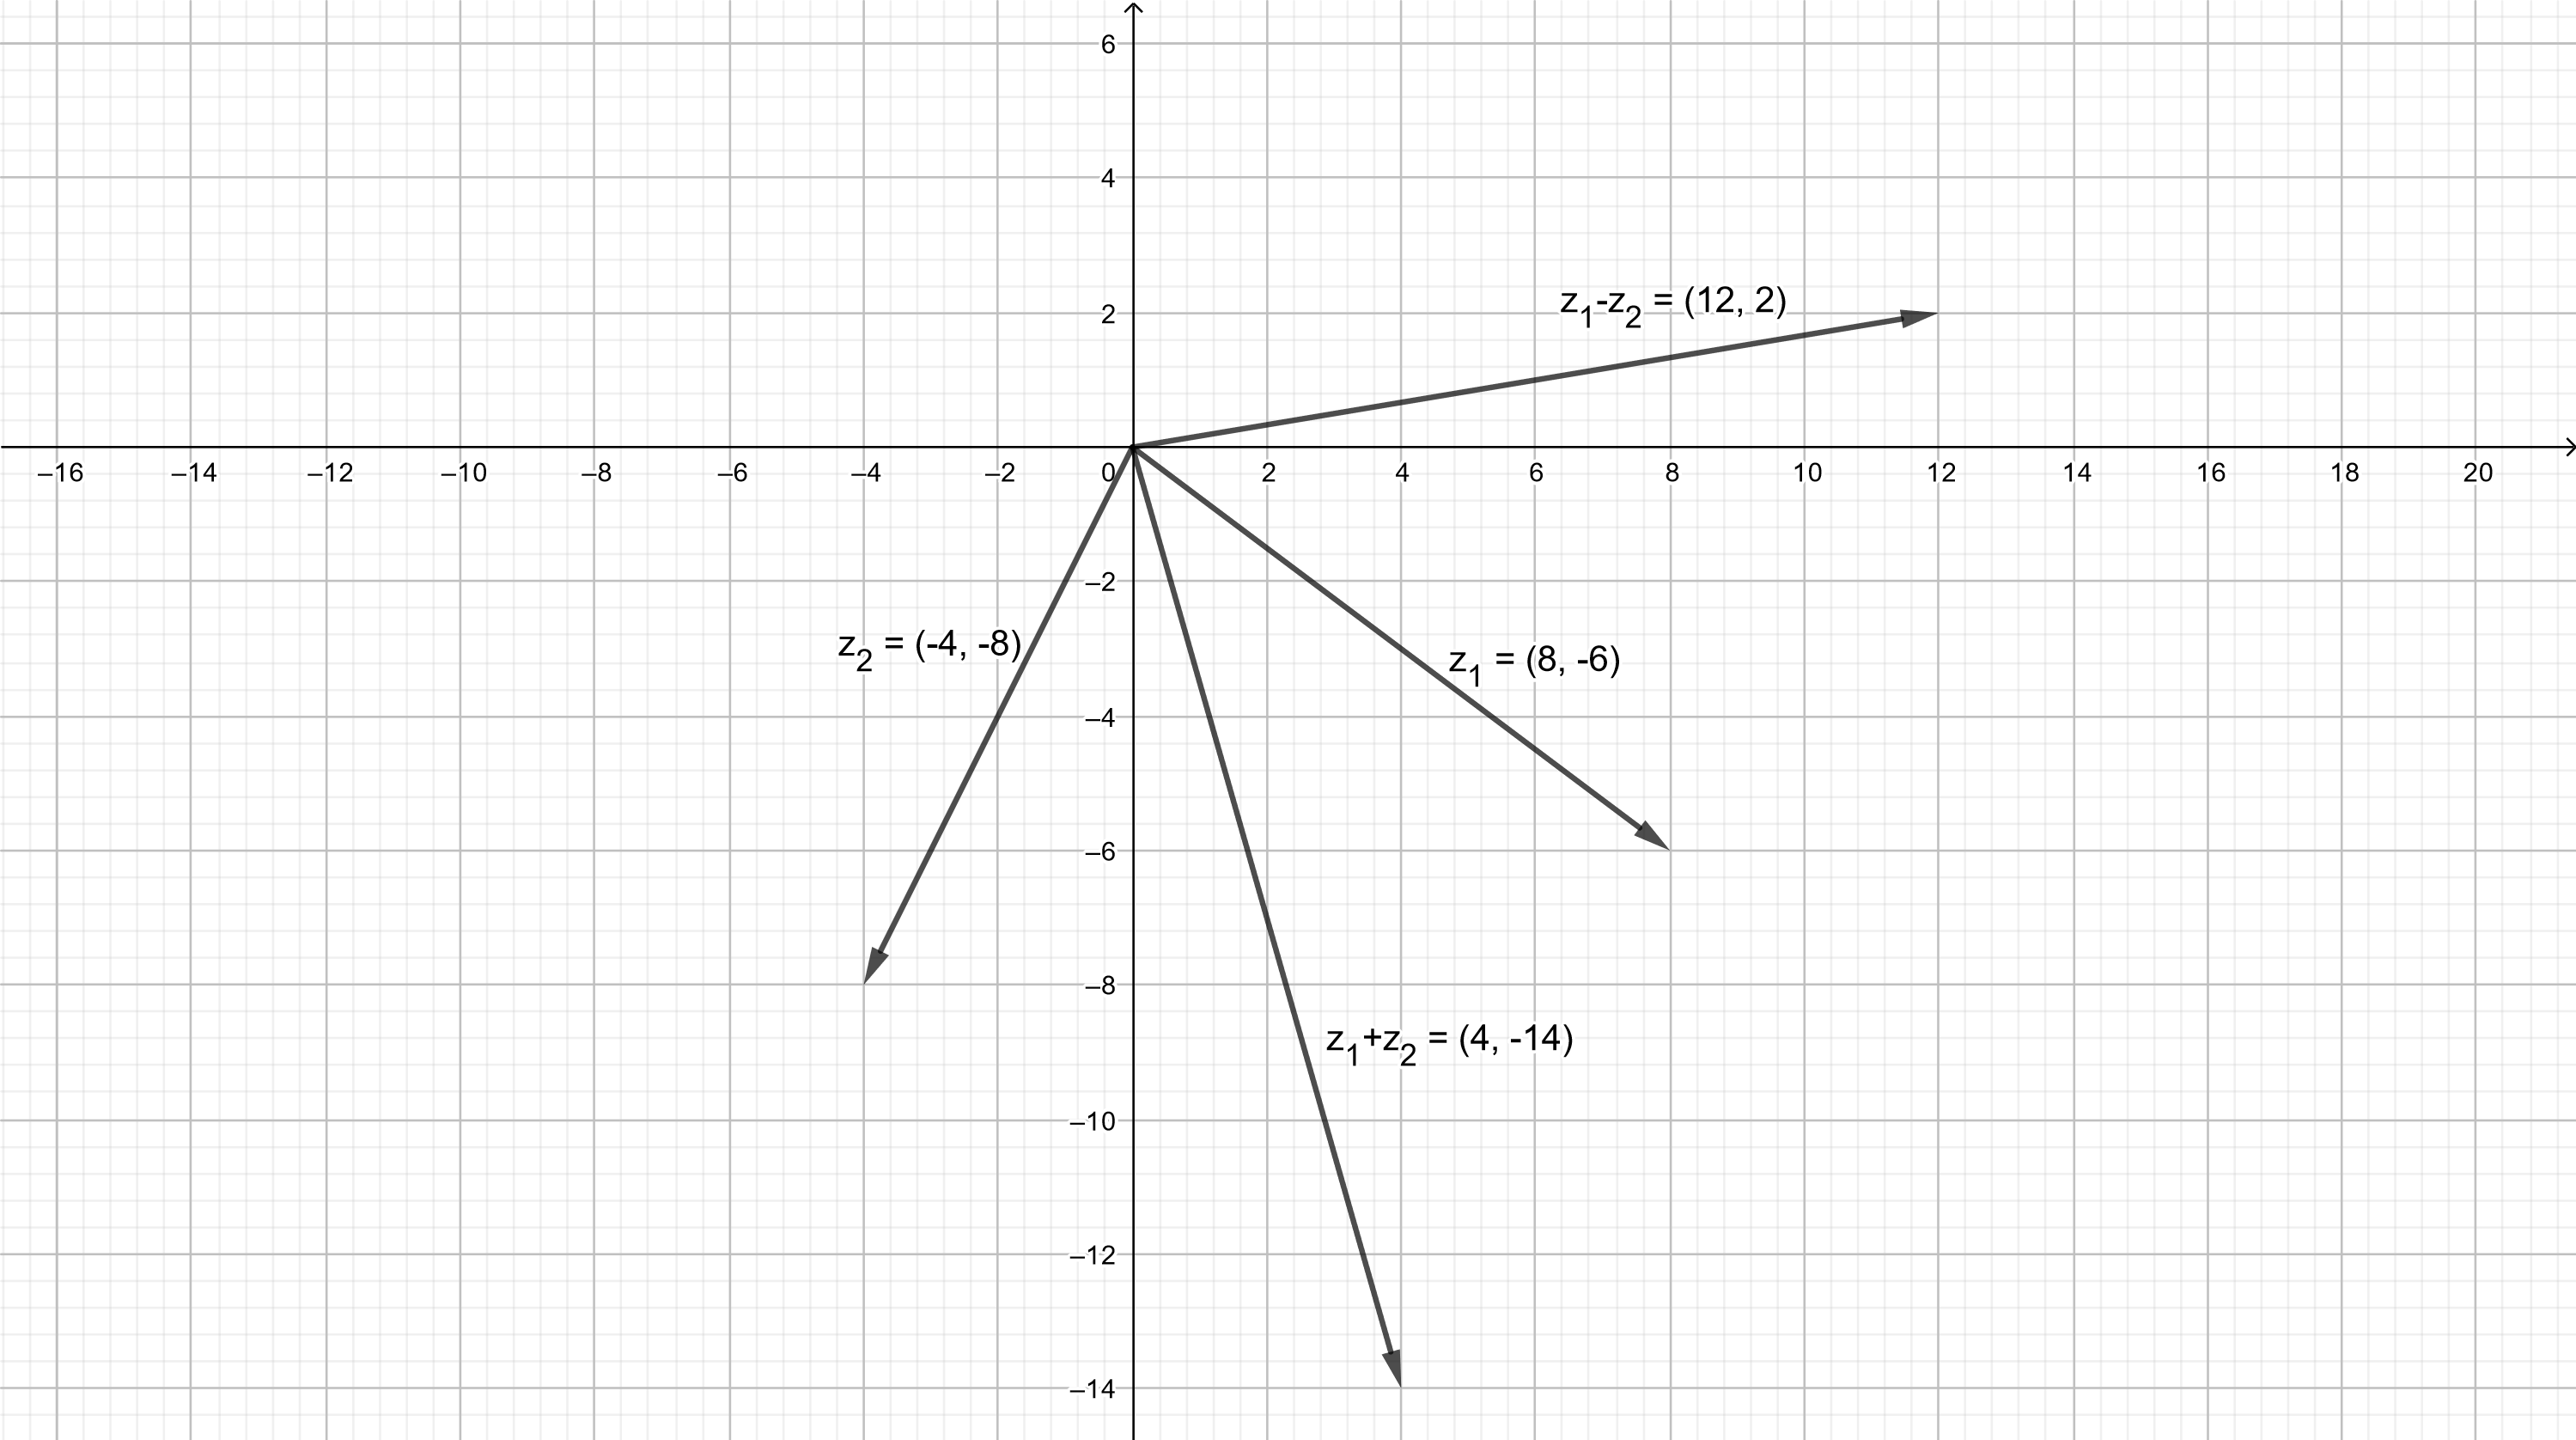
\includegraphics[width=15cm]{geo3}

\begin{center}
\textbf{Operaciones Aritméticas}
\end{center}

En cada uno de los ejercicios \ding{175} al \ding{179} realice las operaciones indicadas simplificando tanto como sea posible (Recuerde que: $\bf{i^{2}\,=\,-\,1}$)\\

\textcolor{ao(english)}{\ding{175}}\,\quad\,$\bf{3\left(-\,1\,+\,4\,i\right)\,-\,2\left(7\,-\,i\right)}$

$$3\left(-\,1\,+\,4\,i\right)\,-\,2\left(7\,-\,i\right)\,=\,-\,3\,+\,12\,i\,-\,\left(14\,-\,2\,i\right)$$

$$=\,\left(-\,3\,-\,14\right)\,+\,i\left(12\,-\,(-\,2)\right)\,=\,-\,17\,+\,i\left(12\,+\,2\right)\,=\,-\,17\,+\,14\,i$$\\

\textcolor{ao(english)}{\ding{176}}\,\quad\,$\bf{\left(i\,-\,2\right)\,\left[2\left(1\,+\,i\right)\,-\,3\left(i\,-\,1\right)\right]}$

$$\left(i\,-\,2\right)\,\left[2\left(1\,+\,i\right)\,-\,3\left(i\,-\,1\right)\right]\,=\,\left(i\,-\,2\right)\,\left[2\,+\,2\,i\,-\,\left(3\,i\,-\,3\right)\right]\,=\,\left(i\,-\,2\right)\,\left[\left(2\,-\,(-\,3)\right)\,+\,i\left(2\,-\,3\right)\right]$$

$$=\,\left(i\,-\,2\right)\,\left[\left(2\,+\,3\right)\,-\,\,i\right]\,=\,\left(-\,2\,+\,i\right)\,\left(5\,-\,\,i\right)\,=\,-\,10\,+\,2\,i\,+\,5\,i\,-\,\underbrace{i^{2}}_{\bf{-\,1}}$$

$$=\,\left(-\,10\,+\,1\right)\,+\,i\left(2\,+\,5\right)\,=\,-\,9\,+\,7\,i$$\\

\textcolor{ao(english)}{\ding{177}}\,\quad\,$\bf{\dfrac{\left(2\,+\,i\right)\,\left(3\,-\,2\,i\right)\,\left(1\,+\,2\,i\right)}{\left(1\,-\,i\right)^{2}}}$\\
\\

\textcolor{ao(english)}{\ding{47}}\,Resolver el numerador:

$$\left[\left(2\,+\,i\right)\,\left(3\,-\,2\,i\right)\right]\,\left(1\,+\,2\,i\right)\,=\,\left[6\,-\,4\,i\,+\,3\,i\,+\,4\right]\,\left(1\,+\,2\,i\right)\,=\,\left(10\,-\,i\right)\,\left(1\,+\,2\,i\right)$$

$$=\,10\,+\,20\,i\,-\,i\,+\,2\,=\,12\,-19\,i$$

\textcolor{ao(english)}{\ding{47}}\,Resolver el denominador: 

$$\left(1\,-\,i\right)^{2}\,=\,1\,+\,2\,(1)\,(-\,i)\,+\,\underbrace{i^{2}}_{\bf{-\,1}}\,=\,-\,2\,i$$

\textcolor{ao(english)}{\ding{47}}\,Dividir:

$$\left(\dfrac{12\,-19\,i}{-\,2\,i}\right)\,\left(\dfrac{2\,i}{2\,i}\right)\,=\,\dfrac{24\,i\,+\,38}{4}\,=\,\dfrac{38}{4}\,+\,\dfrac{24}{4}\,i\,=\,\dfrac{19}{2}\,+\,6\,i$$

\textcolor{ao(english)}{\ding{178}}\,\quad\,$\bf{\left(2\,i\,-\,1\right)^{2}\,\left[\dfrac{4}{1\,-\,i}\,+\,\dfrac{2\,-\,i}{1\,+\,i}\right]}$\\

$$\underbrace{\left(2\,i\,-\,1\right)^{2}}_{\bf{z_{1}}}\,\left[\underbrace{\dfrac{4}{1\,-\,i}}_{\bf{z_{2}}}\,+\,\underbrace{\dfrac{2\,-\,i}{1\,+\,i}}_{\bf{z_{3}}}\right]$$

\textcolor{ao(english)}{\ding{47}}\,Resolver $\bf{z_{1}}$:

$$\left(2\,i\,-\,1\right)^{2}\,=\,-\,4\,+\,2\,(-\,1)\,(2\,i)\,+\,1\,=\,-\,3\,-\,4\,i$$

\textcolor{ao(english)}{\ding{47}}\,Resolver $\bf{z_{2}}$:

$$\left(\dfrac{4}{1\,-\,i}\right)\left(\dfrac{1\,+\,i}{1\,+\,i}\right)\,=\,\dfrac{4\,+\,4\,i}{2}\,=\,2\,+\,2\,i$$

\textcolor{ao(english)}{\ding{47}}\,Resolver $\bf{z_{3}}$:

$$\left(\dfrac{2\,-\,i}{1\,+\,i}\right)\left(\dfrac{1\,-\,i}{1\,-\,i}\right)\,=\,\dfrac{2\,-\,2\,i\,-\,i\,-\,1}{1\,-\,(-\,1)}\,=\,\dfrac{1\,-\,3\,i}{2}\,=\,\dfrac{1}{2}\,-\,\dfrac{3}{2}\,i$$

\textcolor{ao(english)}{\ding{47}}\,Resolver $\bf{z_{2}\,+\,z_{3}}$:

$$2\,+\,2\,i\,+\,\dfrac{1}{2}\,-\,\dfrac{3}{2}\,i\,=\,\dfrac{4\,+\,1}{2}\,+\,\dfrac{4\,-\,3}{2}\,i\,=\,\dfrac{5}{2}\,+\,\dfrac{1}{2}\,i$$


\textcolor{ao(english)}{\ding{47}}\,Resolver $\bf{z_{1}\,\left[z_{2}\,+\,z_{3}\right]}$:

$$\left(-\,3\,-\,4\,i\right)\,\left(\dfrac{5}{2}\,+\,\dfrac{1}{2}\,i\right)\,=\,-\,\dfrac{15}{2}\,-\,\dfrac{3}{2}\,i\,-\,10\,i\,+\,2\,=\,\dfrac{-\,15\,+\,4}{2}\,+\,i\left(\dfrac{-\,3\,-\,20}{2}\right)\,=\,-\,\dfrac{11}{2}\,-\,\dfrac{23}{2}\,i$$\\

\textcolor{ao(english)}{\ding{179}}\,\quad\,$\bf{\dfrac{i^{4}\,+\,i^{9}\,+\,i^{16}}{2\,-\,i^{5}\,+\,i^{10}\,-\,i^{15}}}$\\

$$\dfrac{i^{4}\,+\,i^{9}\,+\,i^{16}}{2\,-\,i^{5}\,+\,i^{10}\,-\,i^{15}}\,=\,\dfrac{1\,+\,i\,+\,1}{2\,-\,i\,-\,1\,+\,i}\,=\,\dfrac{2\,+\,i}{1}\,=\,2\,+\,i$$

\end{document}